\documentclass[10pt]{article}
\usepackage[margin=0.92in]{geometry}
\usepackage{amsmath,amssymb}
\usepackage{booktabs}
\usepackage{graphicx}
\usepackage{cite}
\usepackage{tikz}
\usetikzlibrary{positioning,arrows.meta}
\usepackage{setspace}
\setstretch{1.12}

\title{An Illumination-Invariant Chromatic Prototype Head\\ for Identifying Beer-Crate Colors}
\author{Computer Science\\ System Design and Optimization}
\date{}

\begin{document}
\maketitle

\begin{abstract}
A side camera at a brewery warehouse gate must name each beer crate by body color while a forklift carries the stack past. The plastic face is nearly one reflectance, so a classical color-constancy correction divides that reflectance away and the type is lost. This paper attaches a small chromatic prototype head to a YOLO-style instance segmenter. Inside each mask the head builds an eight-dimensional feature from corrected chromaticity, opponent color, and the chromaticity of a shades-of-gray illuminant estimate, then scores six learned prototypes. On a Monte Carlo face model the classical corrections stay near chance. The head is slightly behind raw color matching under a nearly white lamp and ahead of it once the illuminant severity grows, at a cost of $9760$ parameters. Amber and yellow, $9.3^{\circ}$ apart in the design palette, remain the confused pair.
\end{abstract}

\noindent\textbf{Keywords---}color constancy, instance segmentation, prototype classifier, crate identification.

\section{Introduction}
The last visual check in this packaging line is not a bottle. It is a pallet of returnable crates on a forklift, seen from the side as the truck enters the warehouse. The inventory needs a count per body color. Color here is a stock-keeping unit: amber, green, red, blue, yellow, and white in the palette used below. The lamp is not under the designer's control. Dock daylight and interior lamps change the observed RGB of a face that is otherwise uniform.

Two standard answers fail for opposite reasons. A classifier on raw RGB memorizes the product of illuminant and reflectance, and the decision moves when the truck uses another door. A gray-world or shades-of-gray correction~\cite{buchsbaum1980,finlayson2004} assumes a mixture of reflectances. On one plastic face the estimate is parallel to the observed color, the corrected face is driven toward gray, and the type disappears. Global white balance has the same defect at frame scale: the floor and the safety paint vote on a gain that is not the light on any one crate~\cite{gijsenij2011,afifi2019}.

The head proposed here, the illumination-invariant chromatic prototype head (ICPH), does not emit a corrected image. It emits a class and a margin for each instance mask. Corrected chromaticity is kept only as a residual that is informative when the mask is contaminated. The illuminant estimate is kept as its own coordinates, because that is where the reflectance still sits after a uniform face has been ``corrected.'' A linear layer on the concatenation is enough for six prototypes. The segmenter is unchanged except for this head.

The numbers below are estimates under a stated generator of faces, not a filmed aisle. They are the evidence available without gate images, and they are labeled as such.

\section{Related work}
Computational color constancy estimates a single illuminant so that a photograph can be rendered as if under a white lamp~\cite{gijsenij2011}. The Minkowski family includes gray-world at order $p=1$ and shades-of-gray at a moderate order, commonly six~\cite{buchsbaum1980,finlayson2004}. Edge-based variants move the norm onto derivatives so that large flat surfaces do not dominate~\cite{vandeweijer2007}. Learned estimators pool local guesses with a confidence~\cite{hu2017} or reduce the problem to localization in the Fourier domain~\cite{barron2017}. All of them are built for scenes that contain many reflectances. A crate mask is the case they exclude.

Recognition networks lose accuracy when the input white balance is wrong~\cite{afifi2019}, which is why a locked camera gain is a reasonable installation choice. Locking the gain does not by itself name the plastic. The naming still has to be trained across lamps.

Instance segmentation supplies the mask. YOLACT assembles a mask as a linear combination of shared prototypes~\cite{bolya2019}, and the YOLO segmentation line uses that assembly~\cite{jocher2023}. Those spatial prototypes are not color prototypes. Reusing the mask coefficients as a color code would entangle the seam between two crates with the lamp. ICPH therefore reads pixels inside the mask, not the coefficient vector.

\section{Method}
\subsection{What must not be classified}
Under a diagonal illuminant model~\cite{gijsenij2011}, a shaded face of one reflectance is
\begin{equation}
\mathbf{I}(x)=s(x)\,\mathbf{L}\odot\mathbf{R},\qquad x\in M,
\label{eq:diag}
\end{equation}
with $M$ the predicted mask, $\mathbf{L}$ a positive illuminant, and $\mathbf{R}$ constant on the body. If the shade $s$ is also constant, every Minkowski norm of $\mathbf{I}$ on $M$ is parallel to $\mathbf{L}\odot\mathbf{R}$. Dividing by that norm yields a neutral chromaticity. The correction has succeeded at removing the lamp and, in the same division, at removing the class. ICPH therefore does not classify the corrected color.

The residual that a classifier can use comes from violations of that ideal: a shade ramp, a logo, and a strip of the neighboring crate where the mask is a few pixels too wide. Those signals are weak. The strong signal on a clean face is the chromaticity of the norm itself, which still points at $\mathbf{L}\odot\mathbf{R}$.

\subsection{Feature and scores}
On $M$, with order $p=6$,
\begin{equation}
\hat\ell_c=\Big(\frac{1}{|M|}\sum_{x\in M}|I_c(x)|^6\Big)^{1/6}.
\label{eq:sog}
\end{equation}
Corrected pixels are $\mathbf{I}'=\mathbf{I}\oslash\hat\ell$. Let $\chi$ be the chromaticity of their mean, $o=(\chi_r-\chi_g,\ \tfrac12(\chi_r+\chi_g)-\chi_b)$ the opponent pair, and $\eta$ the chromaticity of $\hat\ell$. The feature is the concatenation $\mathbf{f}=[\chi;o;\eta]\in\mathbb{R}^{8}$. Training coordinates are standardized. Class scores are linear, $z=W\tilde{\mathbf{f}}+b$, and the prediction is $\operatorname{argmax}_k z_k$. The margin between the best score and the second best is retained so the system can abstain. The training loss is cross-entropy plus $\lambda\|W\|_F^2$ with $\lambda=10^{-3}$.

The design reflectances, as linear RGB triples, are amber $(0.72,0.45,0.12)$, green $(0.15,0.55,0.22)$, red $(0.70,0.12,0.12)$, blue $(0.12,0.25,0.62)$, yellow $(0.85,0.75,0.15)$, and white $(0.82,0.82,0.80)$. They are separable by construction and are not a spectrophotometer record of a named crate. The cosine of amber and yellow is $0.987$, an angle of about $9.3^{\circ}$. Red and blue sit near $67^{\circ}$. A lamp perturbation of about fourteen degrees, the root-mean-square scale of severity $0.30$ derived below, is already larger than the amber--yellow gap.

\begin{figure}[t]
\centering
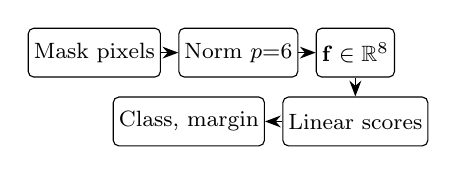
\begin{tikzpicture}[
  font=\footnotesize,
  box/.style={draw, rounded corners=2pt, align=center, inner sep=2pt, minimum height=6.2mm},
  arr/.style={-{Stealth}, semithick}
]
\node[box] (m) {Mask pixels};
\node[box, right=2.2mm of m] (s) {Norm $p{=}6$};
\node[box, right=2.2mm of s] (f) {$\mathbf{f}\in\mathbb{R}^{8}$};
\node[box, below=2.4mm of f] (z) {Linear scores};
\node[box, left=2.2mm of z] (k) {Class, margin};
\draw[arr] (m)--(s);\draw[arr] (s)--(f);\draw[arr] (f)--(z);\draw[arr] (z)--(k);
\end{tikzpicture}
\caption{ICPH on one mask. Corrected chromaticity is not the classifier input by itself. It is one block of $\mathbf{f}$, beside the illuminant chromaticity the correction would have divided out.}
\label{fig:head}
\end{figure}

A full segmenter can also mask-pool a $256$-d neck vector and project it to $32$ dimensions, with a small perceptron on the raw channel means. Counted as specified, that path adds $9760$ weights. Relative to a medium YOLO segmenter of $27.3$ million parameters, the fraction is $3.6\times 10^{-4}$. The Monte Carlo estimate trains only the eight-dimensional linear head. It does not train a backbone. The parameter count is a specification, not a profiled runtime.

\subsection{How a face is drawn}
A class is drawn uniformly. A gain $\mathbf{g}=\exp(\xi)$ has independent normal log-coordinates of standard deviation $s$, then is divided by its mean so that a pure exposure change is not double-counted. A shadow is uniform on $[0.40,1]$, a shade ramp runs from $0.72$ to $1.18$, and with probability $0.25$ the first $18\%$ of the rows are replaced by another prototype under the same gain. Pixel noise has standard deviation $0.012$. For small $s$ the root-mean-square angle of $\mathbf{g}$ from white is $s\sqrt{2/3}$: about $2^{\circ}$ at $s=0.05$ and about $14^{\circ}$ at $s=0.30$. At $s=0.60$ the linearization fails and a one-standard-deviation log-gain is a factor near $1.8$ between channels.

The raw baseline matches the mean pixel to the nearest prototype by cosine, with no correction. Gray-world and shades-of-gray correct with $p=1$ and $p=6$, then match the same way. Those two are predicted to collapse. Raw matching is predicted to win only while $\mathbf{g}$ is near white.

\section{Estimate}
Six thousand training faces use $s$ uniform on $[0.05,0.55]$ and five hundred full-batch steps at learning rate $0.35$. Each test severity uses $2500$ fresh faces. Top-1 accuracy is the fraction whose predicted class equals the reflectance class, before the gain was applied. The neighbor strip does not change the label.

\begin{table}[t]
\caption{Top-1 accuracy versus illuminant severity. Chance on six classes is $0.167$.}
\label{tab:acc}
\centering
\footnotesize
\setlength{\tabcolsep}{3pt}
\begin{tabular}{@{}lcccc@{}}
\toprule
$s$ & Raw & Gray-world & Shades-of-gray & ICPH \\
\midrule
$0.05$ & $0.986$ & $0.165$ & $0.196$ & $0.972$ \\
$0.15$ & $0.900$ & $0.180$ & $0.211$ & $0.914$ \\
$0.30$ & $0.778$ & $0.186$ & $0.219$ & $0.834$ \\
$0.45$ & $0.618$ & $0.172$ & $0.208$ & $0.687$ \\
$0.60$ & $0.531$ & $0.171$ & $0.204$ & $0.607$ \\
\bottomrule
\end{tabular}
\end{table}

Table~\ref{tab:acc} matches the prediction. Both classical corrections stay between $0.165$ and $0.219$ at every severity. Raw matching leads at $s=0.05$ ($0.986$ against $0.972$) and is behind from $s=0.15$ onward. The gap at the harsh end is $0.076$, from $0.531$ to $0.607$. That is a real lead and not a solved problem. At $s=0.60$, per-class recall is $0.47$ amber, $0.67$ green, $0.78$ red, $0.81$ blue, $0.41$ yellow, and $0.50$ white. Amber sends many faces to yellow and yellow sends many back. White's errors spread across the chromatic classes, which is what a near-neutral prototype does when $\hat\ell$ is noisy.

A second run from the same seed, with the random stream consumed in subset order, isolates coordinates. Chromaticity alone, or opponent color alone, stays near $0.48$--$0.55$. The illuminant block alone reaches $0.864$ at $s=0.05$ and falls to $0.504$ at $s=0.60$. Chromaticity plus illuminant matches the full vector within a few thousandths. Opponent axes are almost redundant under an $\ell_2$ penalty. They are kept because they cost two coordinates and because the amber--yellow direction is an opponent direction. The ablation says the decision is not ``invariant'' by living in corrected chromaticity. Corrected chromaticity is the weak block. The class is carried by $\eta$ together with the residual that contamination leaves in $\chi$.

\section{How the head is used}
The camera white balance is locked for the shift. Firmware automatic white balance is a global gain of the kind rejected above, and it moves when the mast of the truck enters the frame. Once a week, a set of known-color pallets records the distribution of margins. Faces below the tenth percentile of that distribution are listed for a person and are not forced into a color tally. The total geometric count does not depend on the margin. A low-margin amber face is a naming question, not a reason to discard the stack count.

The operating rule follows the table rather than a slogan. Under a mild lamp, raw matching is enough and slightly better. Under a lamp the weekly margins show to be strong, ICPH is the better of the two and still must abstain, first on amber and yellow. Under either lamp, correcting and then matching is not a competitor.

\section{What this estimate does not say}
The generator draws one face at a time. It does not render a logo as a spatial pattern, a specular highlight on wet plastic, or a camera whose automatic white balance is still hunting. Those are reasons a gate trial can move the numbers. They are not reasons to go back to dividing a uniform face by its own mean. The neck-pooled path counted in the parameter budget is specified so a later training run has somewhere to put a printed logo. It was not trained here, and the accuracies above must not be quoted as if it had been.

A second limit is the palette. The $9.3^{\circ}$ gap between amber and yellow is a property of the six design triples. A factory palette whose nearest colors sit farther apart would make the same linear layer look more accurate without any change in the algorithm. The confusion matrix, not the mean, is the number a deployment should recompute on its own crates.

\section{Conclusion}
Naming a uniform colored face is not the color-constancy problem. The correction that removes the lamp also removes the only reflectance in the mask. ICPH keeps that reflectance inside the illuminant feature, keeps the corrected color only as a residual, and scores six prototypes with a linear layer small enough to ignore in a segmenter budget. On the face generator, classical per-mask constancy falls to chance, and the head's advantage over raw color appears when the lamp leaves the white point and grows only into the mid sixties at the harshest severity. A gate trial would replace the severity dial with the building's own lamps and would publish the confusion matrix, not only the mean.

\begin{thebibliography}{99}
\bibitem{buchsbaum1980} G.~Buchsbaum, ``A spatial processor model for object colour perception,'' \emph{J. Franklin Institute}, vol.~310, no.~1, pp.~1--26, 1980.
\bibitem{finlayson2004} G.~D.~Finlayson and E.~Trezzi, ``Shades of gray and colour constancy,'' in \emph{Color and Imaging Conf.}, 2004, pp.~37--41.
\bibitem{gijsenij2011} A.~Gijsenij, T.~Gevers, and J.~van de Weijer, ``Computational color constancy: Survey and experiments,'' \emph{IEEE Trans. Image Process.}, vol.~20, no.~9, pp.~2475--2489, 2011.
\bibitem{vandeweijer2007} J.~van de Weijer, T.~Gevers, and A.~Gijsenij, ``Edge-based color constancy,'' \emph{IEEE Trans. Pattern Anal. Mach. Intell.}, vol.~29, no.~4, pp.~687--700, 2007.
\bibitem{hu2017} Y.~Hu, B.~Wang, and S.~Lin, ``FC4: Fully convolutional color constancy with confidence-weighted pooling,'' in \emph{CVPR}, 2017, pp.~4085--4094.
\bibitem{barron2017} J.~T.~Barron and Y.-T.~Tsai, ``Fast Fourier color constancy,'' in \emph{CVPR}, 2017, pp.~886--894.
\bibitem{afifi2019} M.~Afifi and M.~S.~Brown, ``What else can fool deep learning? Addressing color constancy errors on deep neural network performance,'' in \emph{ICCV}, 2019, pp.~243--252.
\bibitem{bolya2019} D.~Bolya, C.~Zhou, F.~Xiao, and Y.~J.~Lee, ``YOLACT: Real-time instance segmentation,'' in \emph{ICCV}, 2019, pp.~9157--9166.
\bibitem{jocher2023} G.~Jocher, A.~Chaurasia, and J.~Qiu, ``YOLO by Ultralytics,'' software release, 2023.
\bibitem{oh2017} S.~W.~Oh and S.~J.~Kim, ``Approaching the computational color constancy as a classification problem through deep learning,'' arXiv:1608.07951, 2017.
\end{thebibliography}

\end{document}
